\renewcommand\evenpagerightmark{{\scshape\small Experiment results}}
\chapter[Experiment results]%
{Experiment results}
\label{experiment_chapt}

\section{Objectives}


\subsection{Accuracy of visible image }

This section shows all the difficulties occurring when camera are used as diagnostic with high accuracy expectancies.  When taking the picture of an image, the signal will 
depend linearly on the ISO sensibility and the exposure time. Hence, before any results or interpretation one must testify that the 
post processing and the results does not depend on the acquisition parameters at all. Otherwise, 
the given flame length would not be reliable and no interpretation or comparison could be drawn. 
Unfortunately, the best solution would have been to choose to reason at the same acquisition parameters (ISO/exposure time), 
but this solution does not work at all for serveral reasons :

\begin{itemize}
\item The acquisition parameters of the main flame to be compared with (Freiberg flame) are not known, even raw images are not provided in the internship
\item With the same acquisition paramers, a flame without soot (mainly blue) will produce a very poor signal (ISO has then to be increased), whereas a flame with much soot will be so bright that the exposure time has to be drastically reduced in order to protect the sensor and not to have a fully saturated image
\end{itemize}

This point is fairly stressed, as a major work has been conducted to provide results and post processing which do not depend on the acquisition parameters.

Here are the results of N flame, which is the Freiberg scaled flame on Calhory. A sensitivity analysis has been conducted, with ISO varying from 100 to 4000 and exposure time from 1/30 to 1/400. The images are RGB averaged from movies of 10 seconds. Here extreme examples of the signal that can be obtained of the same flame with different acquisition parameters.

\subsection{The impossibility to match the curves with different parameters acquisition}

The purpose here is to find similarities between the signals of different acquisition parameters to define a flame length. Hence, here is the intensity signal along the axis of the flame, on a 1D curve for a better comparison, on the figure on the left. The different curves correspond to different acquisition parameters. 

The shapes of the signal is comparable for all the acquisition parameters, except when the signal is saturated. Unfortunately, for every curve, there is a point where the signal reaches zero. And this points increases when the ISO sensibility increases. That zero values impedes from properly re-sizing. On the right picture, the signal of the whole picture has been uniformed to go from 1 o  signal. One can see that the zero value still gives major difference between the curves. Hence, one can easily see that a thresh method as Otsu's method is inefficient to define a proper flame length. (the small blue curve would give 200 pixels and orange curve would give 500 pixels). 

My opinion is that the pictures taken by the camera are coded from 0 to 255, and that an image with a small ISO sensibility will give strict 0 value in the non flame area, and and a small value if the ISO is high. Consequently, even with multiplying the signal to uniform the curves, the 0 value will remain 0, and there is no possibility to match the curves.
\begin{figure}[h!]
  \centering
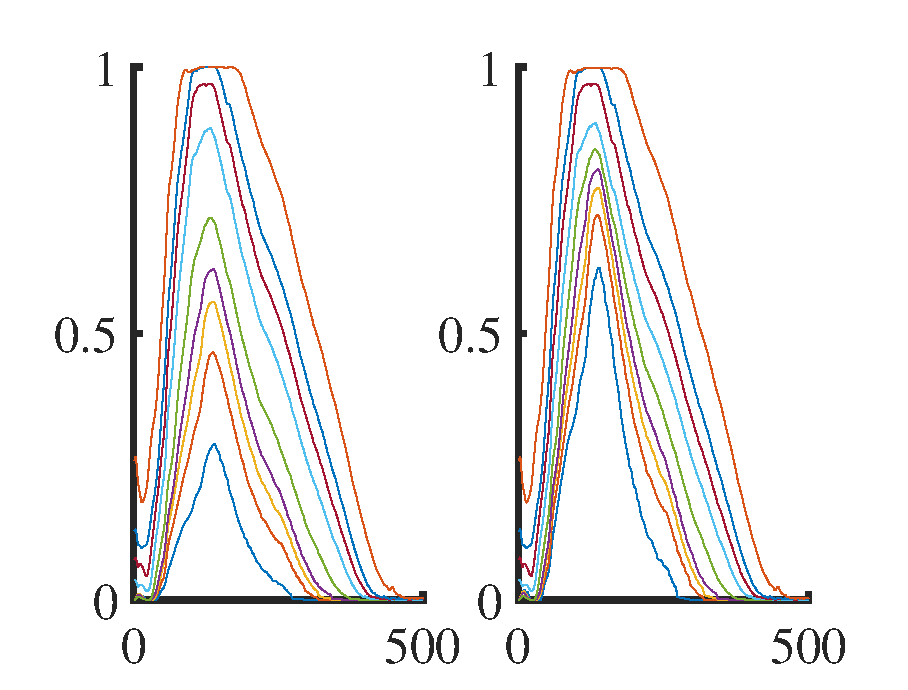
\includegraphics[width=0.60\textwidth]{fig/Signal_comparison.eps}

  \caption{Signal on the axis of the burner of the averaged movies, the different curves corresponding to different acquisition parameters. Left : Original, Right : signal uniformed from 0  to 1}
 \label{signal_comparison}
\end{figure}
What can be stressed is that the maximum point of each curves is always found at the same position  : 135 pixels. With the current observation, the point where the signal is maximum is here the only geometric parameters that does not depend on the acquisition parameters. On figure \ref{contour}, the post processed image of the flame are shown : from top to bottom, the ISO sensibility is increasing but they all represent the same flame. This results is just a confirmation in 2D of the 1D curve in figure \ref{signal_comparison}. One can also see that the Odsu's threshold in white gives a flame length that increases quasi linearly with the ISO sensibility.

On the right, ten iso contours are drawn for the corresponding photos. What can be seen is that, at the same abscissa $x=100px$, the shape of the contour changes of convexity (for $x <100px$ there is a backward curved contour, that cannot be see for $x>100px$). What matters the most is that this edge can be seen at the same position in every parameter acquisition (except for the last at the bottom, which is totally saturated).

\begin{figure}[h!]
  \centering
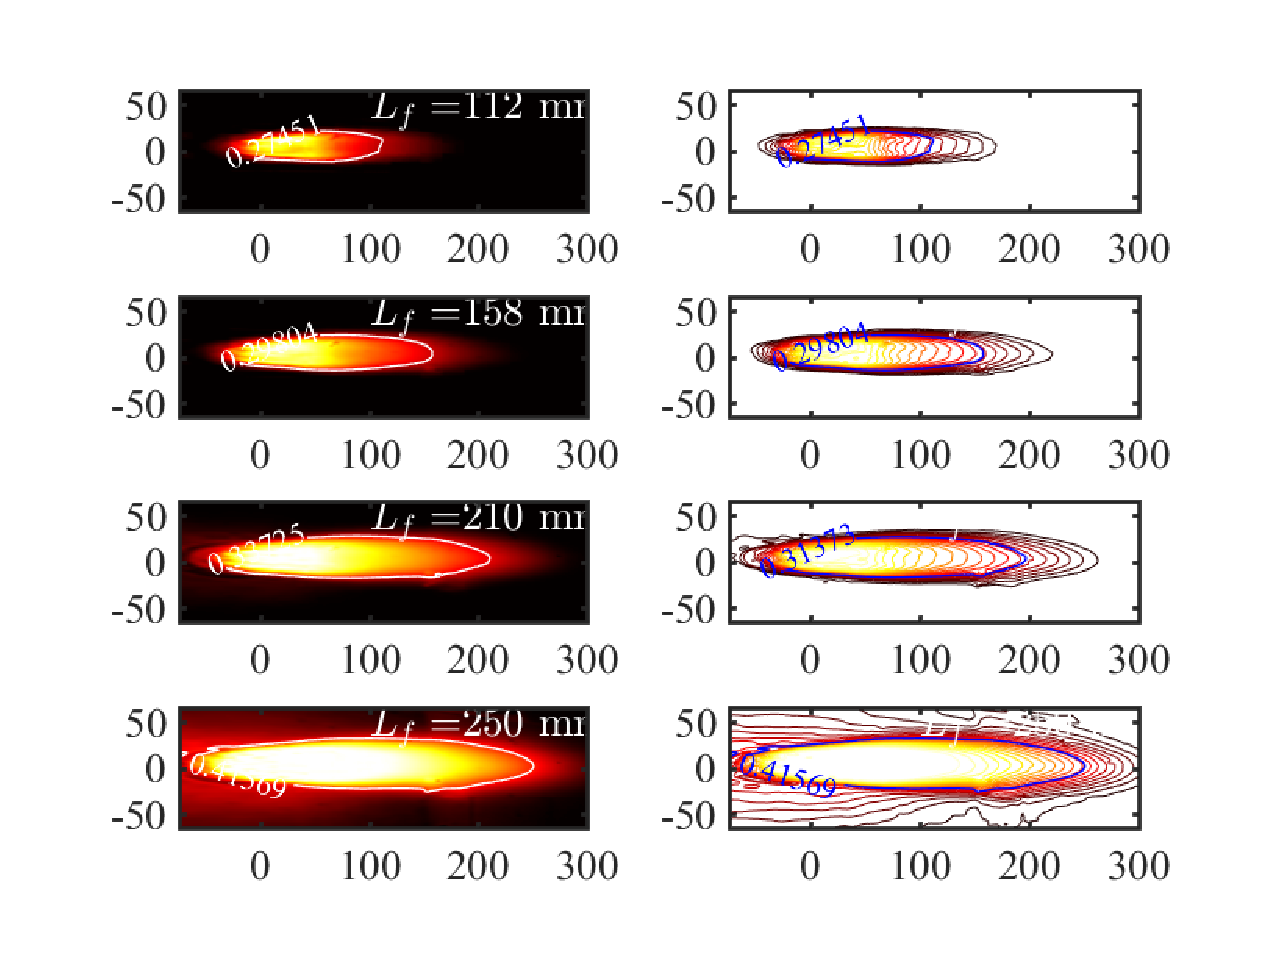
\includegraphics[width=1\textwidth]{fig/Contour.eps}

  \caption{Post processed flames, left : images, right : contours, from top to bottom, the ISO sensibility increases}
 \label{contour}
\end{figure}


\subsection{Comparison between chimiluminescence and visible image}

\begin{figure}[h!]
  \centering
\includegraphics[width=1\textwidth]{fig/Comparaison_chimil.jpg}

  \caption{On the top : visible image, on the bottom, chimiluminescence}
 \label{contour}
\end{figure}
\subsection{The flame topology does depend on the adimensional identified number }
The figure \label{fig_power_comparison} shows that as it is expected in \#ref Veynantes, the flame length is not driven by the Reynolds number, in the
turbulent case.
 \begin{figure}[!h]
  \centering
\includegraphics[width=0.3\textwidth]{fig/puissance/DSC_3683puissance.png}
\includegraphics[width=0.3\textwidth]{fig/puissance/DSC_3689puissance.png}
\includegraphics[width=0.3\textwidth]{fig/puissance/DSC_3694puissance.png}
  \caption{Three different Reynolds number flame with same topology}
 \label{fig_power_comparison}
\end{figure}



\section{Results on Freiberg burner}
\subsubsection{The flame can be well reproduced}
\subsubsection{Parametric analysis}

\section{Results on prototype burner}
\subsubsection{The burner works perfectly}
\subsubsection{Permits to understand more the importance of impulsion ratio and swirl number}
\subsubsection{The Swirl is relevant only if the momentum of the jet is of importance}